\documentclass{article}

\usepackage[utf8x]{inputenc}
\usepackage{ucs}
\usepackage[portuguese]{babel}
\usepackage[T1]{fontenc}
\usepackage{amsmath}
\usepackage{amsfonts}
\usepackage{amssymb}
\usepackage{graphicx}
\usepackage{fancyhdr}
\usepackage{lastpage}
\usepackage{geometry}
\usepackage{float}
\usepackage{makecell}
\usepackage{multirow}
%\usepackage{subfigure}
\usepackage[table,xcdraw]{xcolor}
\usepackage{caption}
\usepackage{subcaption}
\usepackage{cases}
%\usepackage[framed,numbered,autolinebreaks,useliterate]{matlab-prettifier}
%\usepackage{mcode}
%\usepackage{filecontents}
\graphicspath{{Imagens/}}

% Mudando a fonte do documento para Times New Roman (ptm)
\renewcommand*\rmdefault{ptm}

\pagestyle{fancy}
\fancyhf{}
\lhead[]{Redes Neurais Artificiais}
\rhead[]{Relatório I}
\chead[]{}

\lfoot{Página \thepage \enspace de \pageref{LastPage} }
\rfoot{\leftmark}
\renewcommand{\footrulewidth}{1pt}

\usepackage{Sweave}
\begin{document}
\Sconcordance{concordance:Relatorio_1.tex:Relatorio_1.Rnw:%
1 39 1 1 0 26 1 1 2 1 0 1 1 1 2 6 0 1 2 4 1}


\begin{center}

{\scshape\Large Universidade Federal de Minas Gerais \par}
{\scshape\large Redes Neurais Artificiais \par}
\vspace{5cm}

\hrule
\hfill

{\huge \textbf{Perceptron e Adaline}\par}
\hfill
\hrule
\hfill

\vspace{3cm}

{\large\itshape Victor Marcius Magalhães Pinto\\Mat: 2019717730\par}

\vspace{2cm}

\end{center}

\newpage

\section{Introdução}

Os exercícios pro;...

\section{Classificação}

\subsection{Classes linearmente separáveis}
\begin{Schunk}
\begin{Sinput}
> class1 = matrix(rnorm(400, 3, 1), ncol = 2)
> class2 = matrix(rnorm(400, 7, 1), ncol = 2)
\end{Sinput}
\end{Schunk}

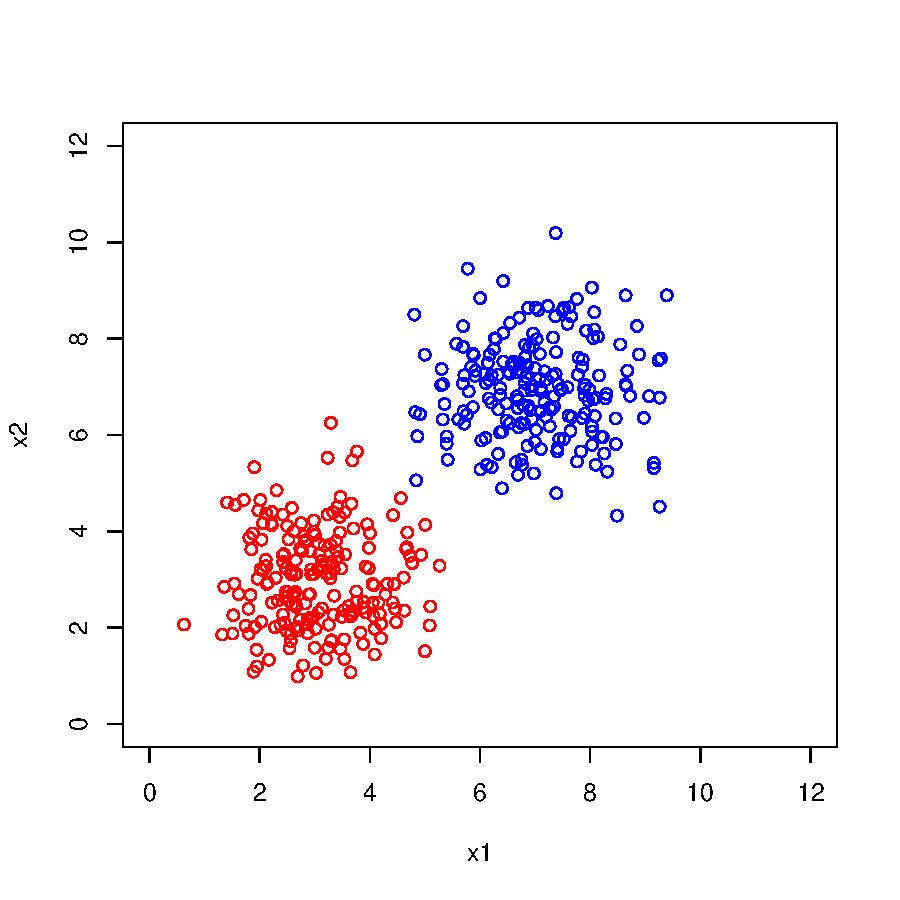
\includegraphics{Relatorio_1-002}


\begin{Schunk}
\begin{Sinput}
> ydata = read.csv("BUILDING1paraR.DT", sep=" ")
\end{Sinput}
\end{Schunk}




\end{document}
